% Vector schematic of the HEFEL loop redrawn from Smolik et al. (FFHMT 2023), Fig. 2 (left).
% Not to scale; the published source is cited in the dissertation caption.
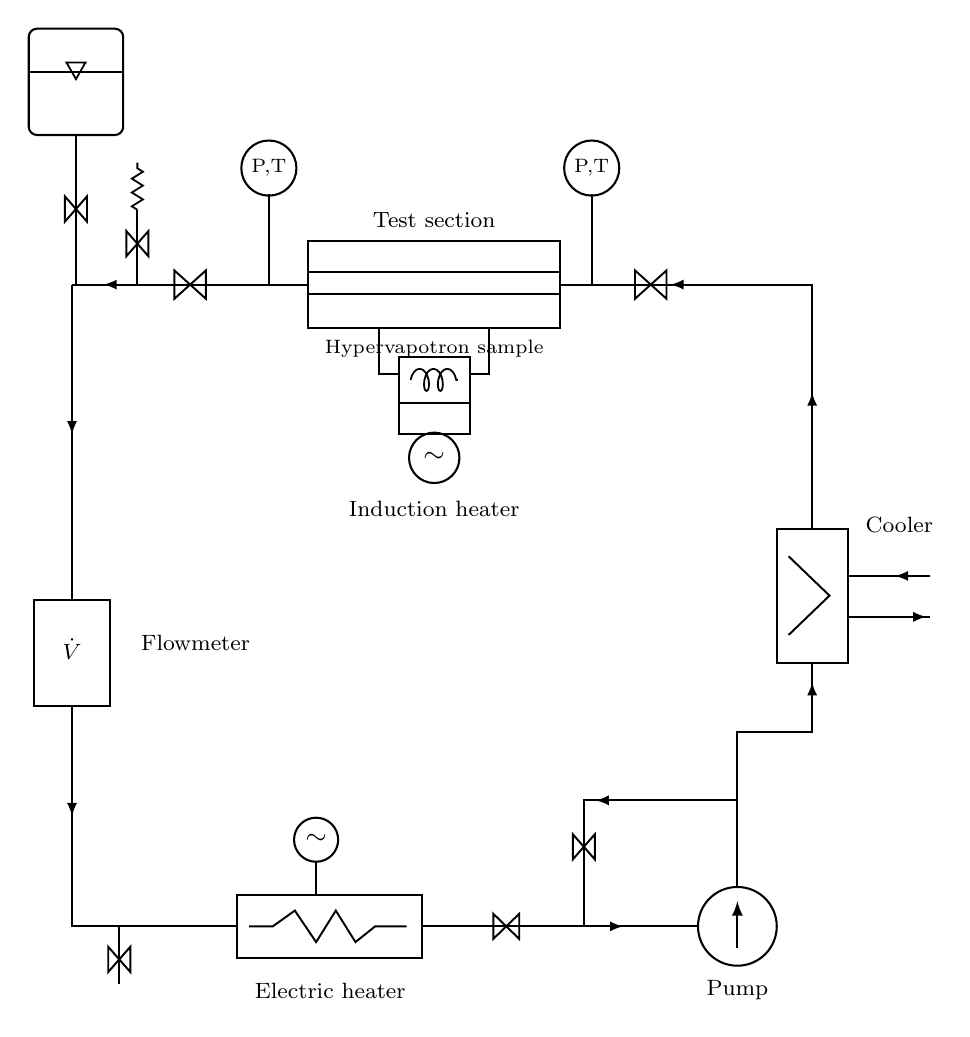
\begin{tikzpicture}[x=1cm,y=1cm,line width=.65pt,>=latex,
 pipe/.style={line width=.7pt},
 component/.style={draw,line width=.75pt},
 lab/.style={font=\footnotesize},
 smalllab/.style={font=\scriptsize}]
% test section and pipework
\draw[pipe] (1.4,10) -- (4.4,10);
\draw[component] (4.4,9.45) rectangle (7.6,10.55);
\draw (4.4,10.16) -- (7.6,10.16);
\draw (4.4,9.88) -- (7.6,9.88);
\draw[pipe] (7.6,10) -- (10.8,10) -- (10.8,6.9);
\node[lab,above] at (6,10.6) {Test section};
\node[smalllab,below] at (6,9.43) {Hypervapotron sample};
% pressure and temperature gauges
\draw (3.9,10) -- (3.9,11.15);
\draw[component] (3.9,11.48) circle (.35);
\node[smalllab] at (3.9,11.48) {P,T};
\draw (8,10) -- (8,11.15);
\draw[component] (8,11.48) circle (.35);
\node[smalllab] at (8,11.48) {P,T};
% valves near test section
\draw[pipe] (2.7,9.82) -- (3.1,10.18) -- (3.1,9.82) -- (2.7,10.18) -- cycle;
\draw[pipe] (8.55,9.82) -- (8.95,10.18) -- (8.95,9.82) -- (8.55,10.18) -- cycle;
% induction heater
\draw[pipe] (5.3,9.45) -- (5.3,8.86) -- (5.55,8.86);
\draw[pipe] (6.7,9.45) -- (6.7,8.86) -- (6.45,8.86);
\draw[component] (5.55,8.5) rectangle (6.45,9.08);
\draw[decorate,decoration={coil,aspect=.5,segment length=5pt,amplitude=4pt}] (5.7,8.79) -- (6.3,8.79);
\draw[pipe] (5.55,8.5) -- (5.55,8.1) -- (6,8.1);
\draw[pipe] (6.45,8.5) -- (6.45,8.1) -- (6,8.1);
\draw[component] (6,7.8) circle (.32);
\node[font=\normalsize] at (6,7.8) {$\sim$};
\node[lab,below] at (6,7.38) {Induction heater};
% flowmeter
\draw[pipe] (1.4,10) -- (1.4,6.0);
\draw[component] (.92,4.65) rectangle (1.88,6.0);
\node[lab,anchor=west] at (2.15,5.45) {Flowmeter};
\node[lab] at (1.4,5.37) {$\dot{V}$};
\draw[pipe] (1.4,4.65) -- (1.4,1.85) -- (3.5,1.85);
\draw[->] (1.4,8.55) -- (1.4,8.1);
\draw[->] (1.4,3.65) -- (1.4,3.25);
% electric heater and AC supply
\draw[component] (3.5,1.45) rectangle (5.85,2.25);
\draw[pipe] (3.65,1.85) -- (3.95,1.85) -- (4.23,2.05) -- (4.5,1.65) -- (4.75,2.05) -- (5.0,1.65) -- (5.25,1.85) -- (5.65,1.85);
\node[lab,below] at (4.68,1.26) {Electric heater};
\draw[pipe] (4.5,2.25) -- (4.5,2.65);
\draw[component] (4.5,2.95) circle (.28);
\node at (4.5,2.95) {$\sim$};
\draw[pipe] (5.85,1.85) -- (9.35,1.85);
\draw[pipe] (6.75,1.69) -- (7.08,2.01) -- (7.08,1.69) -- (6.75,2.01) -- cycle;
\draw[->] (7.9,1.85) -- (8.4,1.85);
% pump
\draw[component] (9.85,1.85) circle (.5);
\draw[->,thick] (9.85,1.58) -- (9.85,2.17);
\node[lab,below] at (9.85,1.29) {Pump};
\draw[pipe] (9.85,2.35) -- (9.85,4.32) -- (10.8,4.32) -- (10.8,5.2);
% cooler
\draw[component] (10.35,5.2) rectangle (11.25,6.9);
\draw[pipe] (10.5,5.55) -- (11.02,6.05) -- (10.5,6.55);
\node[lab,right] at (11.35,6.95) {Cooler};
\draw[pipe] (11.25,6.3) -- (12.3,6.3);
\draw[pipe] (11.25,5.78) -- (12.3,5.78);
\draw[->] (12.3,6.3) -- (11.85,6.3);
\draw[->] (11.82,5.78) -- (12.25,5.78);
\draw[->] (10.8,8.2) -- (10.8,8.63);
\draw[->] (10.8,4.53) -- (10.8,4.95);
% bypass
\draw[pipe] (9.85,3.45) -- (7.9,3.45) -- (7.9,1.85);
\draw[pipe] (7.76,2.7) -- (8.04,3.02) -- (8.04,2.7) -- (7.76,3.02) -- cycle;
\draw[->] (8.5,3.45) -- (8.05,3.45);
% expansion tank and relief
\draw[component,rounded corners=3pt] (.85,11.9) rectangle (2.05,13.25);
\draw (.85,12.7) -- (2.05,12.7);
\draw (1.57,12.82)--(1.45,12.61)--(1.33,12.82)--cycle;
\draw[pipe] (1.45,11.9) -- (1.45,10);
\draw[pipe] (1.31,10.8)--(1.59,11.12)--(1.59,10.8)--(1.31,11.12)--cycle;
\draw[pipe] (2.23,10) -- (2.23,10.95);
\draw[pipe] (2.09,10.36)--(2.37,10.68)--(2.37,10.36)--(2.09,10.68)--cycle;
\draw[decorate,decoration={zigzag,segment length=5pt,amplitude=2pt}] (2.23,10.95)--(2.23,11.55);
% drain and upper flow
\draw[pipe] (2,1.85) -- (2,1.12);
\draw[pipe] (1.86,1.27)--(2.14,1.59)--(2.14,1.27)--(1.86,1.59)--cycle;
\draw[->] (9.45,10) -- (9,10);
\draw[->] (2.2,10) -- (1.8,10);
\end{tikzpicture}
